\documentclass{llncs}
\usepackage{times}
\usepackage[T1]{fontenc}

% Comentar para not MAC Users
%\usepackage[applemac]{inputenc}

\usepackage{a4}
%\usepackage[margin=3cm,nohead]{geometry}
\usepackage{epstopdf}
\usepackage{indentfirst}
\usepackage{graphicx}
\graphicspath{{Capturas-Ecra/}}
\usepackage{float}
\usepackage{fancyvrb}
\usepackage{amsmath}
\usepackage{array}
%\renewcommand{\baselinestretch}{1.5}


\begin{document}
\mainmatter
\title{TP1 - Protocolos da Camada de Transporte}

\titlerunning{TP1 - Protocolos da Camada de Transporte}

\author{Diogo Braga \and João Silva}

\authorrunning{Diogo Braga \and João Silva}

\institute{
University of Minho, Department of  Informatics, 4710-057 Braga, Portugal\\
e-mail: \{a82547,a82005\}@alunos.uminho.pt\\
PL2, Grupo 6
}

\date{}
\bibliographystyle{splncs}

\maketitle

\section{Questão 1}

\begin{center}
\begin{tabular}{ | m{3cm} | m{3cm} | m{3cm} | m{3cm} | m{3cm} |}
\hline
 \textbf{Comando usado (aplicação)} & \textbf{Protocolo de Aplicação(se aplicável)} & \textbf{Protocolo de transporte(se aplicável)} & \textbf{Porta de atendimento(se aplicável)} & \textbf{Overhead de transporte em bytes(se aplicável)} \\
 \hline
 \textbf{Ping} & -------------------------- & -------------------------- & -------------------------- & -------------------------- \\
 \hline
 \textbf{traceroute} & -------------------------- & -------------------------- & -------------------------- & -------------------------- \\
 \hline
 \textbf{telnet} & Telnet & TCP & 23 & 20 \\
 \hline
 \textbf{ftp} & FTP & TCP & 21 & 32 \\
 \hline
 \textbf{Tftp} & TFTP & UDP & 69 & 22 \\
 \hline
 \textbf{browser/http} & HTTP & TCP & 80 & 32 \\
 \hline
 \textbf{nslookup} & DNS & UDP & 53 & 47 \\
 \hline
 \textbf{ssh} & SSH & TCP & 22 & 32 \\
 \hline
\end{tabular}
\end{center}

\subsection{Ping}

\begin{figure}[H]
\begin{center}
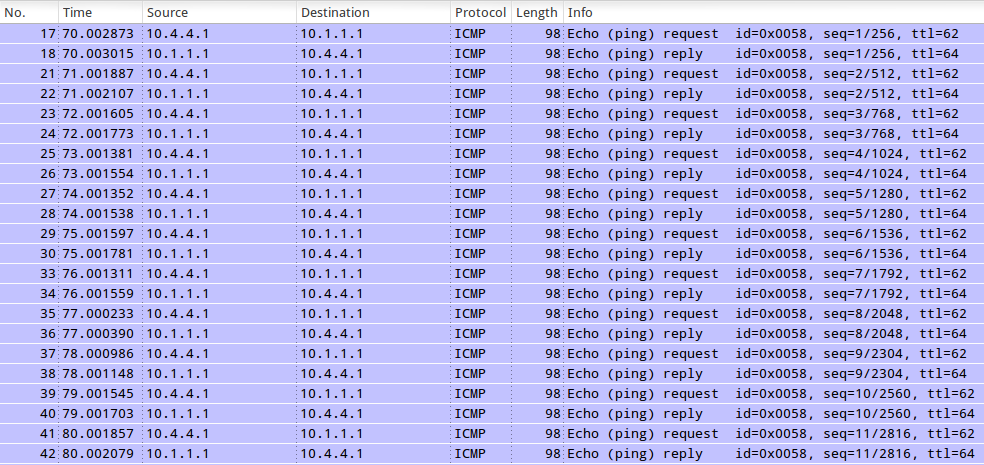
\includegraphics[scale=0.4]{ping.png}
\end{center}
\caption{\label{fig:ping}Captura realizada aquando a realização do comando \emph{ping}.}
\end{figure}

Como possível reparar na figura \ref{fig:ping}, o comando \emph{ping} apenas utiliza \textbf{ICMP} pelo que atua praticamente apenas no nível de rede, daí as nossas escolhas aquando do preenchimento do quadro.


\subsection{Traceroute}

\begin{figure}[H]
\begin{center}
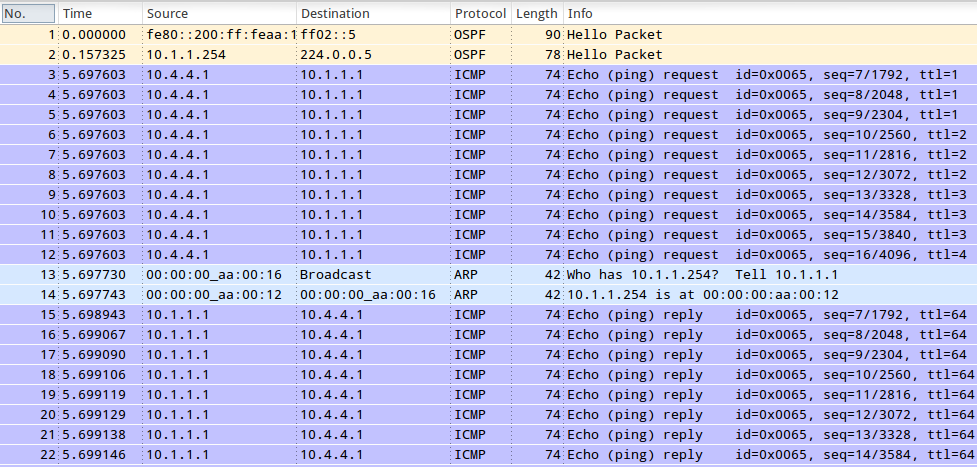
\includegraphics[scale=0.4]{traceroute.png}
\end{center}
\caption{\label{fig:traceroute}Captura realizada aquando a realização do comando \emph{traceroute}.}
\end{figure}

Como possível reparar na figura \ref{fig:traceroute}, o comando \emph{traceroute}, tal como o \emph{ping}, apenas utiliza \textbf{ICMP} pelo que atua praticamente apenas no nível de rede, daí as nossas escolhas aquando do preenchimento do quadro.


\subsection{Telnet}

\begin{figure}[H]
\begin{center}
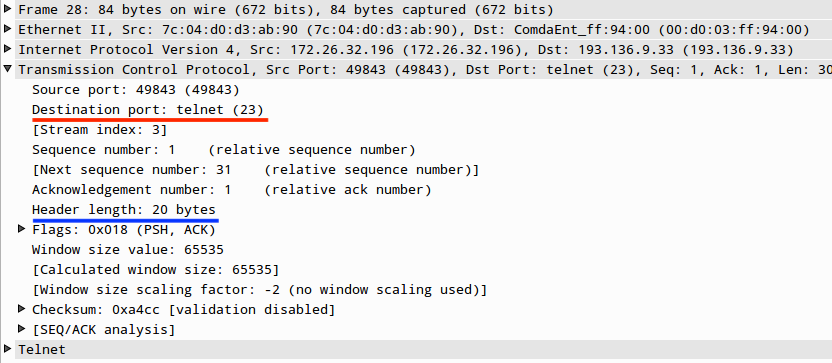
\includegraphics[scale=0.4]{telnet.png}
\end{center}
\caption{\label{fig:telnet}Captura realizada aquando a realização do comando \emph{telnet}.}
\end{figure}

A figura \ref{fig:telnet}, representa um Frame capturado que contém um cabeçalho referente à aplicação \textbf{Telnet}. Deste modo na camada de transporte (TCP) conseguimos identificar a porta de atendimento bem como o overhead de transporte em bytes, que se encontram a sublinhado na figura \ref{fig:telnet}.


\subsection{FTP}

\begin{figure}[H]
\begin{center}
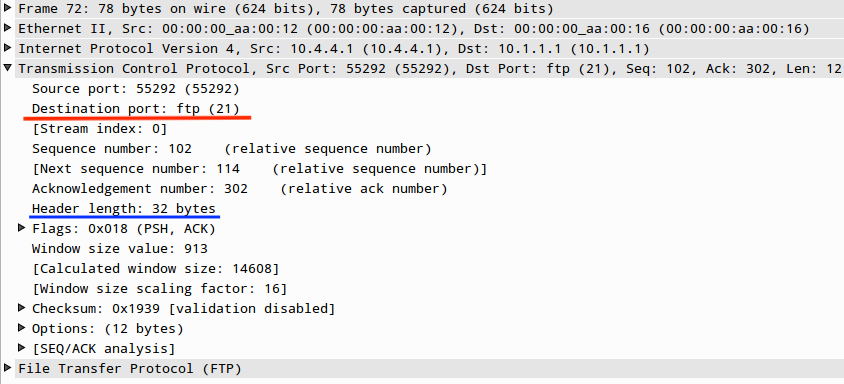
\includegraphics[scale=0.4]{ftp.png}
\end{center}
\caption{\label{fig:ftp}Captura realizada aquando a utilização do protocolo \emph{FTP}.}
\end{figure}

A figura \ref{fig:ftp}, representa um Frame capturado que contém um cabeçalho referente à aplicação \textbf{FTP}. Deste modo na camada de transporte (TCP) conseguimos identificar a porta de atendimento bem como o overhead de transporte em bytes, que se encontram a sublinhado na figura \ref{fig:ftp}.


\subsection{TFTP}

\begin{figure}[H]
\begin{center}
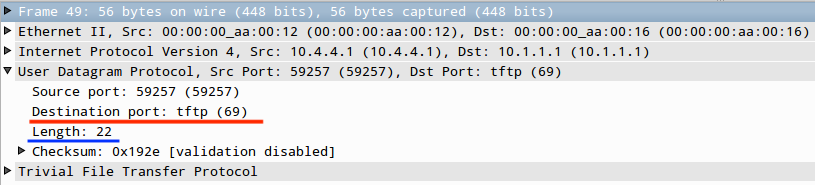
\includegraphics[scale=0.4]{tftp.png}
\end{center}
\caption{\label{fig:tftp}Captura realizada aquando a utilização do protocolo \emph{TFTP}.}
\end{figure}

A figura \ref{fig:tftp}, representa um Frame capturado que contém um cabeçalho referente à aplicação \textbf{FTP}. Deste modo na camada de transporte (UDP) conseguimos identificar a porta de atendimento bem como o overhead de transporte em bytes, que se encontram a sublinhado na figura \ref{fig:ftp}.


\subsection{HTTP}

\begin{figure}[H]
\begin{center}
\includegraphics[scale=0.4]{http.png}
\end{center}
\caption{\label{fig:http}Captura realizada aquando a utilização do protocolo \emph{HTTP}.}
\end{figure}

A figura \ref{fig:http}, representa um Frame capturado que contém um cabeçalho referente à aplicação \textbf{HTTP}. Deste modo na camada de transporte (TCP) conseguimos identificar a porta de atendimento bem como o overhead de transporte em bytes, que se encontram a sublinhado na figura \ref{fig:ftp}.


\subsection{Nslookup}



\subsection{SSH}

\begin{figure}[H]
\begin{center}
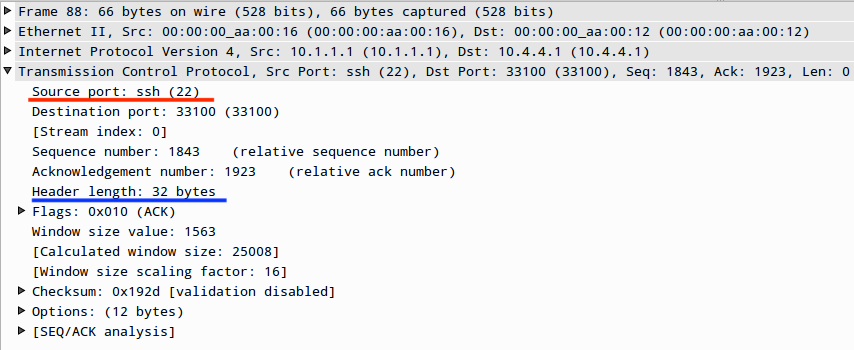
\includegraphics[scale=0.4]{ssh.png}
\end{center}
\caption{\label{fig:ssh}Captura realizada aquando a utilização do protocolo \emph{SSH}.}
\end{figure}

A figura \ref{fig:ssh}, representa um Frame capturado que contém um cabeçalho referente à aplicação \textbf{SSH}. Deste modo na camada de transporte (TCP) conseguimos identificar a porta de atendimento bem como o overhead de transporte em bytes, que se encontram a sublinhado na figura \ref{fig:ssh}.


\section{Questão 2}

Nas duas figuras seguintes, o endereço 10.1.1.1 identifica o Servidor1 da LAN1, e o endereço 10.4.4.1 identifica o Cliente1, host da LAN4 da topologia em causa.

\begin{figure}[H]
\begin{center}
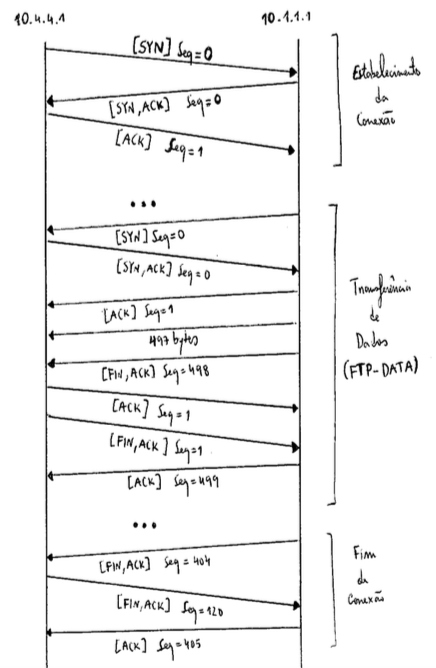
\includegraphics[scale=0.45]{2_ftp.png}
\end{center}
\caption{\label{fig:ssh}Diagrama temporal das transferências do file1 por FTP.}
\end{figure}

\begin{figure}[H]
\begin{center}
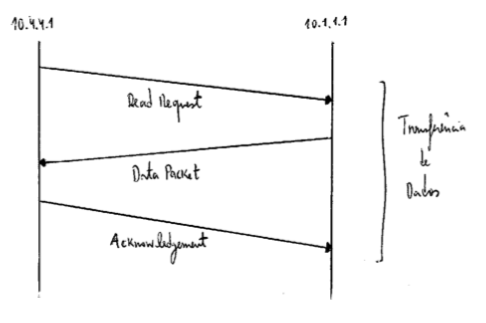
\includegraphics[scale=0.45]{2_tftp.png}
\end{center}
\caption{\label{fig:ssh}Diagrama temporal das transferências do file1 por TFTP.}
\end{figure}

\section{Questão 3}
\subsection{(i) uso da camada de transporte}
Perante os resultados obtidas na Questão 1, podemos concluir que, tanto o FTP, como o HTTP e o SSH utilizam o TCP como camada de transporte, enquanto o TFTP utiliza o UDP para essa função.

Isto leva-nos a concluir que no TFTP existe um menor controlo do envio dos dados por parte da camada de transporte, visto este ser antes controlado pela camada de aplicação.

Nas restantes aplicações em causa, como é usado o TCP sabemos que o transporte, sendo orientado à conexão, é realizado de uma forma mais fiável.

\subsection{(ii) eficiência na transferência}
No protocolo de aplicação TFTP, como é usado UDP, não há estabelecimento e terminação da conexão o que deixa menos garantias de que a transferência seja realizada (eficientemente/com sucesso)(????????).

Nos restantes três protocolos de aplicação, devido ao uso do TCP, a transferência é mais fiável, pois são efetuadas conexões lógicas, existindo em cada conexão um par de sockets. Este protocolo de transporte efetua também controlo de erros, de fluxo e de congestão, o que torna a transferência mais segura.

\subsection{(iii) complexidade}
Perante o observado, por exemplo na Questão 2, concluimos que a complexidade de usar o UDP é consideravelmente inferior à de usar o TCP. Nesse caso, o FTP necessita de estabelecer conexão, transferir os dados, e realizar a desconexão. Ainda na mesma questão, conseguimos concluir que o TFTP, através do UDP, apenas realiza a transferência dos dados.

...

\subsection{(iv) segurança}


\section{Questão 4}

\section{Conclusões}

\end{document}
